%Thesis Tempate for Brock University
%Joseph A. Brown
%Permission is Granted to the Department of Computer Science to use this for their own purposes
%No Waranty is Given, Implied or Explicit
%READ THE MANUAL that Graduate Studies Provides and don't blame me

\documentclass[12pt,oneside,openany]{book}
\setlength{\parskip}{\baselineskip}%
\setlength{\parindent}{0pt}%

\usepackage{setspace}
\usepackage{amsmath, amsthm, amssymb}
\usepackage{verbatim, appendix}
\usepackage{graphicx, subfigure}
\usepackage{ulem}
\usepackage{pgfplots}
\usepackage{algorithm}
\usepackage{algorithmic}
\usepackage{graphicx}
\usepackage{tabu}
\usepackage{color}
%feel free to add here

\usepackage[top=1.0in, bottom=1.0in, left=1.5in, right=1.0in]{geometry} %set page margins

\onehalfspacing


\newtheorem{thm}{Theorem}[section]
\newtheorem{cor}[thm]{Corollary}
\newtheorem{lem}[thm]{Lemma}

\begin{document}
\normalem 

%these are added at the end
%libary Release Form
%Examining Committee Sig pages

%Title Page
% \thispagestyle{empty}

\begin{quote}``Your Plastic Pal Who's Fun To Be With.''\end{quote} --- from the marketing division of the Sirius Cybernetics Corporation. 
 %this is the quote page. comment out if you don't have one

\begin{titlepage}
\begin{center}

{\LARGE {\bf Modeling Metal Protein Complexes from}}
\\[0.2cm]{\LARGE {\bf Experimental Extended X-ray }}
\\[0.2cm]{\LARGE {\bf Absorption Fine Structure}}
\\[0.2cm]{\LARGE {\bf using Computational Intelligence}}
\\[3cm]
{\Large{ \bf Collin Price}}
\\[0.5cm]
{\large Department of Computer Science}
\\[3cm]
{\large Submitted in partial fulfillment\\
of the requirements for the degree of}
\\[1cm]
{\large Master of Science}
\\[1cm]
{\large Faculty of Mathematics and Science, Brock University\\
St. Catharines, Ontario}
\\[4cm]
\copyright Collin Price, 2014

\end{center}
\end{titlepage}



%these are not to be numbered
\frontmatter
\pagestyle{empty}

%comment out what you don't need

% %\thispagestyle{empty}
Cool quote?
\thispagestyle{empty}
\section*{Abstract}
\begin{doublespace}
Experimental Extended X-ray Absorption Fine Structure (EXAFS) spectra carry information about the chemical structure of metal protein complexes. However, predicting the structure of such complexes from EXAFS spectra is not a simple task. Currently methods such as Monte Carlo optimization or simulated annealing are used in structure refinement of EXAFS. These methods have proven somewhat successful in structure refinement but have not been successful in finding the global minima.

Multiple population based algorithms, including a genetic algorithm, a restarting genetic algorithm, differential evolution, and particle swarm optimization, are studied for their effectiveness in structure refinement of EXAFS. The oxygen-evolving complex in S$_{1}$ is used as a benchmark for comparing the algorithms. These algorithms were successful in finding new atomic structures that produced improved calculated EXAFS spectra over atomic structures previously found.

\end{doublespace}   


% \thispagestyle{empty}
\section*{Preface}
The Sirius Cybernetics Corporation is "a bunch of mindless jerks who'll be the first against the wall when the revolution comes." An edition of the Encyclopaedia Galactica that had the good fortune to fall through a time warp from a thousand years in the future defined the Sirius Cybernetics Corporation as "a bunch of mindless jerks who were the first against the wall when the revolution came." Note: We would welcome applications from anyone interested in taking over the post of robotics correspondent. 
\thispagestyle{empty}
\section*{Acknowledgements}

% Here I thank all the people!

First and foremost, I would like to thank my supervisor, Dr. Sheridan Houghten for being the best mentor I could have asked for. Without her guidance and patience I would not have been able to achieve the success I have today. I would also like to thank my advisory committee Dr. Doug Bruce, Dr. Brian Ross, and external examiner Dr. Dan Ashlock.

Special thanks goes to the Brock University Computer Science Department. Especially, Donna Phelps for her help navigating the paper work and Cale Fairchild for taking the time to ensure that my experiments ran smoothly and efficiently.

I would like to show my appreciation for Sergey Vassiliev. He helped with the understanding of the biological background and was a vital asset in the success of this work.

Finally, I would like to thank my friends and family, especially Gary and Cathie Price. They supported and motivated me during my research. Without their continuous support I would not be the person I am today.

\begin{flushright}
\textbf{C.P.} %Your initials
\end{flushright}


 
%this is the Table of Contents and other lists.
\thispagestyle{empty}
\pagestyle{empty}
\tableofcontents
\thispagestyle{empty}
\pagestyle{empty}
\clearpage
\listoftables
\thispagestyle{empty}
\pagestyle{empty}
\listoffigures

%%list of Plates
%list of symbols, nonmenclature, or Abbrevations


\mainmatter 
\pagestyle{headings}
\chapter{Introduction}

The aim of this thesis is to find a better method for determining the atomic structure of a molecule using Extended X-Ray Absorption Fine Structure (EXAFS). The thesis uses the oxygen-evolving complex (OEC) in state S$_{1}$ as an example for structure refinement but the developed process can be applied to any given chemical structure that has undergone x-ray absorption spectroscopy experimentation. In this chapter, we introduce the biological background and terms, followed by the problem definition, and finally elaborate on the computer science theories applied to the problem.

\section{Biological Background}

Photosystem II~\cite{oxygenicPhotosynthesis} is the protein complex responsible for the first stage of photosynthesis. Photosynthesis is a process used by plants and other organisms to convert light (photons) into energy. Photons, that are captured from the Sun or other light sources, and water are processed through a water-oxidizing enzyme known as the oxygen-evolving complex (OEC)~\cite{yano2006manganese}. The water molecule (H$_{2}$O) is split into two parts, O$_{2}$ and H$^{+}$. The O$_{2}$ is released from the system, and the H$^{+}$ will be stored and used as a source of energy.

The OEC complex performs oxidation on two water molecules through a series of intermediary states. The ``S-State Cycle''~\cite{yano2006manganese} consists of 5 states: S$_{0}$, S$_{1}$, S$_{2}$, S$_{3}$, and S$_{4}$. During the transition between each state a hydrogen electron is released. After S$_{4}$ concludes O$_{2}$ is formed. For the purpose of this work, the resting or so-called storage state S$_{1}$ will be analysed. The atomic structure of the OEC molecule is altered between each state.

The most significant feature of this compound is its inorganic core, which is \linebreak Mn$_{4}$Ca$_{1}$O$_{x}$Cl$_{1-2}$(HCO$_{3}$)$_{y}$. It is not found anywhere else in biology and is an important biological blueprint for water spliting. By studying OEC the hope is to understand how the oxidation of water can occur at such a low energy cost. Aquiring a better understanding of how the water splitting process occurs will assist in creating biomimetic catalysts or engineered PSII enzymes for real world applications. A visualization of the inorganic core of OEC in S$_{1}$ is shown in Figure~\ref{fig:oec-in-s1}. This figure was generated using the Visual Molecular Dynamics software~\cite{vmd}.

\begin{figure}[H]
	\centering
	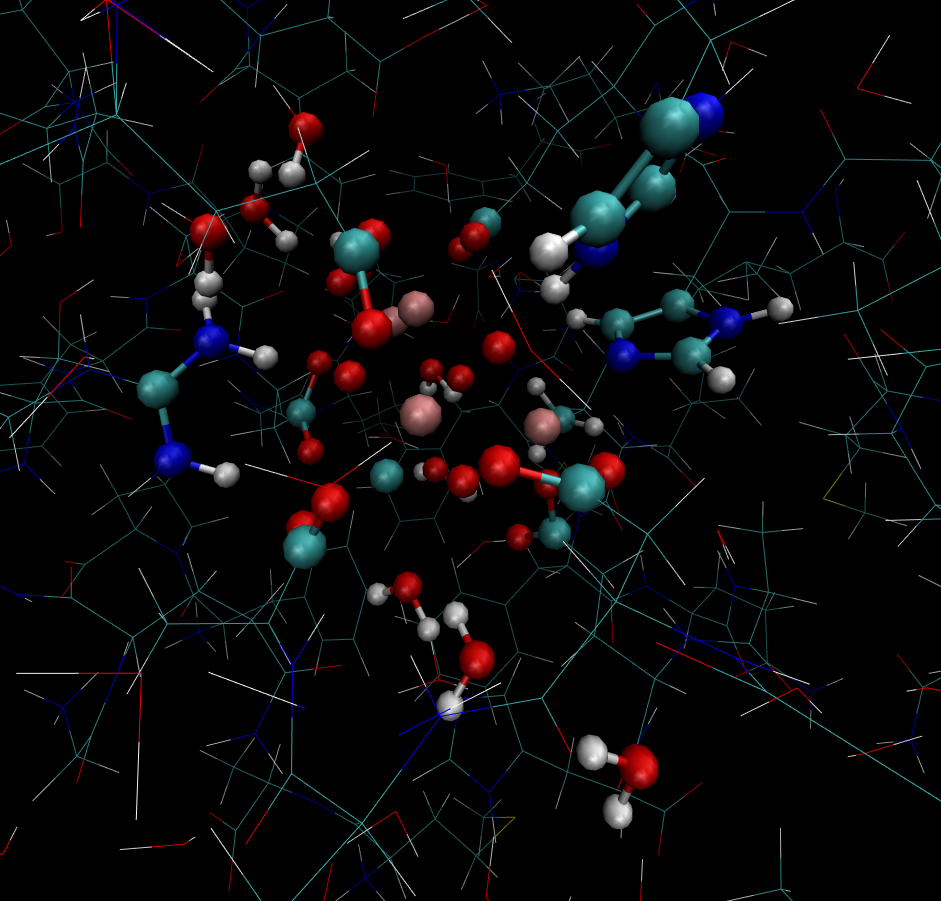
\includegraphics[bb=0 0 941 901,scale=0.3]{figures/structure.png}
	\caption{OEC Atomic Structure in S$_{1}$}
	\label{fig:oec-in-s1}
\end{figure}
\section{X-ray Absorption Spectroscopy}

The following overview is based on information contained in Matthew Newville's \textit{Fundamentals of XAFS} (2004)~\cite{newville2004fundamentals}. X-Ray absorption fine structure (XAFS) is a method used to measure the absorption coefficient of a material as a function of energy. X-rays are part of the electromagnetic spectrum with wavelengths ranging from ~25\AA\ to 0.25\AA. All atoms resonate at a specific wavelength. The x-ray is tuned to have the same wavelength as the target atom. A photon from an x-ray is absorbed by an electron in a tightly bound quantum core level of an atom. Absorption only takes place if the binding energy of the core level is less than the energy of the x-ray photon. At the time of absorption a core electron moves to an empty outer shell and another electron moves in to take its place. Eventually the affected electrons decay to their original state. During this time fluorescence energies are emitted that characterize a specific atom.

The absorption coefficients measured after the initial absorption are referred to as the Extended X-ray Absorption Fine Structure(EXAFS). During the decay of the electrons to their original state, oscillations occur in the measure of the absorption coefficient. The different frequencies found within the oscillations correspond to different near-neighbour coordination shells, which can be described and modeled according to the EXAFS equation. From the oscillations, the number of neighbouring atoms, the distances to the neighbouring atoms, and the disorder in the neighbour distances can be determined. The energy spectrum for OEC in S$_{1}$ is shown in Figure~\ref{fig:oecS1}.

\begin{figure*}
	\begin{tikzpicture}
		\begin{axis}[
			width=14cm,
			height=6cm,
			grid=both,
			title={EXAFS Spectra in k space},
			xlabel={$k \mathbin{/} A\textsuperscript{-1}$},
			ylabel={$EXAFS \chi k\textsuperscript{3}$}
		]

		\addplot[mark=x] table [col sep=comma,y index=1, x index=0] {figures/oec-s1.csv};

		\end{axis}
	\end{tikzpicture}
	\caption{EXAFS Spectra of OEC in S$_{1}$}
	\label{fig:oecS1}
\end{figure*}
\section{Force Fields}

The atoms within a molecule are consistently interacting with each other. Atoms can directly and indirectly interact with neighbouring atoms. Atoms directly interact with neighbouring atoms with a bond or indirectly through van der Waals forces. Calculating the forces involved within the molecule would require a large amount of computing power to attain a high degree of accuracy. Instead simplier, classical formulas are used to calculate the energy within the system. There are several different formulas for calculating classical force fields. This work will utilize Assisted Model Building with Energy Refinement (AMBER)~\cite{cornell1995second} force fields for the energy calculations. AMBER force fields are widely used with proteins and related systems~\cite{ponder2003force}. Equation~\ref{eq:amberFormula} shows the formula used when calculating the energy of a system using AMBER force fields.

\begin{equation}
	\begin{split}
		\label{eq:amberFormula}
		V(r^N) &= \quad \sum_\text{bonds} k_b (l-l_0)^2 \\
		&\quad + \sum_\text{angles} k_a (\theta - \theta_0)^2 \\
		&\quad + \sum_\text{torsions} \sum_n \frac{1}{2} V_n [1+\cos(n \omega- \gamma)] \\
		&\quad + \sum_{j=1} ^{N-1} \sum_{i=j+1} ^N f_{ij}\biggl\{\epsilon_{ij}\biggl[\left(\frac{r_{0ij}}{r_{ij}} \right)^{12} - 2\left(\frac{r_{0ij}}{r_{ij}} \right)^{6} \biggr]+ \frac{q_iq_j}{4\pi \epsilon_0 r_{ij}}\biggr\}
	\end{split}
\end{equation}
\section[Problem Definition: Structure Refinement Problem]{Problem Definition: Structure Refinement\\ Problem}
\label{sec:problem-definition}

The goal of this thesis is to examine different search heuristics to determine the best method of finding the theoretical atomic structure of a molecule using the molecule's EXAFS spectrum for comparison. This problem contains two important but unrelated goals. Firstly, the algorithm must be able to find an atomic structure whose EXAFS spectrum matches the experimental EXAFS spectrum, and secondly, creating an atomic structure whose potential energy is a low as possible.

EXAFS can be used to identify properties of a molecule, but they do not provide enough detail to determine the atomic structure of a molecule in 3-dimensional space. An EXAFS spectrum allows you to identify how far apart atoms are from each other, but does not give enough information to identify their dihedral angles. Fortunately, EXAFS can be used to assist in determining the atomic structure of a molecule. The energy spectrum given off by the molecule is unique to its structure, meaning that you can create an atomic structure, obtain its EXAFS spectrum, and compare the results. The hope is that if you create an atomic structure whose EXAFS spectrum closely matches the EXAFS spectrum of an actual model, then there is a high likelihood that the created structure will closely match the actual structure.

Using EXAFS spectrum comparison the goal is to obtain a set of candidate atomic structures. Atomic structures that generate similar EXAFS spectra may have different geometries. An expert will have to analyse the candidate solutions to determine if any of these atomic structures are actually chemically infeasible. \textbf{Having a set of candidate solutions will improve the odds of finding the actual solution.}

The IFEFFIT XAFS data analysis suite~\cite{ifeffit} is used to simulate the EXAFS experiments. This suite includes two applications that will be used: FEFF6, and IFEFFIT. FEFF6 is used to simulate an XAFS experiment and IFEFFIT does post processing of the simulated EXAFS spectra. During the atomic structure refinement, the generated atomic structures will be run through these applications to obtain an EXAFS spectrum.

NAMD~\cite{namd} will be used for the energy calculations. The NAMD Energy Plugin~\cite{namdEnergy}  will calculate the potential energy of the generated atomic structure.


\section{Thesis Organization}

The remainder of this thesis is organized as follows.
\chapter{Background}

The purpose of this chapter is to assist the reader in understanding the search techniques used in this work. Several different population based search algorithms, including a genetic algorithm, restarting genetic algorithm, differential evolution, and particle swarm optimization are defined in this chapter.

\section{Evolutionary Algorithms}

\subsection{Purpose}



\subsection{Setup}



\subsection{System Parameters}

\begin{table}
	\label{table:ea-pso}
	\centering
	\begin{tabular}{ | >{\bfseries}c | c | c | c | c | c | c | c | c | c | c | c | c | }
		\hline
		Exp. Set & 1 & 2 & 3 & 4 & 5 & 6 & 7 & 8 & 9 & 10 & 11 & 12 \\ \hline
		Pop. Size & 50 & 50 & 50 & 50 & 50 & 50 & 100 & 100 & 100 & 100 & 100 & 100 \\ \hline
		Gens. & 100 & 100 & 100 & 250 & 250 & 250 & 100 & 100 & 100 & 250 & 250 & 250 \\ \hline
		Velocity & 0.01 & 0.05 & 0.1 & 0.01 & 0.05 & 0.1 & 0.01 & 0.05 & 0.1 & 0.01 & 0.05 & 0.1 \\ \hline
	\end{tabular}
	\caption{System parameters for the PSO runs}
\end{table}

\begin{table}
	\label{table:ea-de}
	\centering
	\begin{tabular}{ | >{\bfseries}c | c | c | c | c | }
		\hline
		Experiment Set & 1 & 2 & 3 & 4 \\ \hline
		Population Size & 50 & 50 & 100 & 100 \\ \hline
		Generations & 100 & 200 & 100 & 200 \\ \hline
	\end{tabular}
	\caption{System parameters for the DE runs}
\end{table}

\subsection{Analysis}


% # GA settings

runs: 1
dcd-file: output.dcd.full

# 0 = dcd file, 1 = random
# random required params: max-radius
population-type: 0

population-size: 50
elitism: true
crossover: 0.8
mutation: 0.2
max-generations: 20
results: results.csv

#seed: 1337
xyz-files: benchmark/dft-qm-mm.xyz, benchmark/r-qm-mm.xyz, benchmark/dft-qm-mm2.xyz, benchmark/r-qm-mm2.xyz

# solo, ga, xyz, indexes, index_ga
eval-type: solo
pot-dir: best_chromosomes

index-file: output.dcd.full.csv
# top 200
index-max: 710

# top 300
#index-max: 727

recentering-population: 100
keep-percentage: 0.2
convergence-rate: 0.1
recentering: 3

# DE Config
f: 0.4714
cr: 0.8803

# PSO Config
inertia: 0.729844
social: 1.496180
cognitive: 1.496180
velocity-range: 0.05

\section{Recentering Genetic Algorithm}
\label{sec:rga}

The recentering genetic algorithm (RGA) is a variation of the recentering-restarting genetic algorithm (RRGA)~\cite{hughes2013recentering}~\cite{hughes2013edit} which has had success in avoiding fixation on local optima. RRGA works by performing a series of standard GA runs. Each run uses the final population from the previous run as its starting population with some adjustments. At the beginning of a run the RRGA selects a center, which is a possible candidate solution to the problem, and at the end of each basic GA run the center is compared to the best individual in the population. If the best individual is better than the current center it is replaced with the best individual and the whole process is repeated. The center is used as a baseline for generating the population in the next run.

The RGA works similarly to the RRGA but there is no center for the population. Instead a basic GA is allowed to run until the population's fitness scores begin to converge. After the population has converged upon a minimum diversity, new individuals are introduced to the population. Individuals are considered to be the same if they share the same fitness score. Duplicate individuals are removed from the population and new individuals that have not yet been in any population take their place. For example, if there is a population size of 100 and the convergence rate is 5\% then after all the duplicates are removed there will only be 5 individuals remaining and 95 new individuals will be inserted into the population. Algorithm~\ref{alg:restartingPopulation} shows the pseudo-code of the restarting method.

\begin{algorithm}[H]
\caption{Restarting the population}
\label{alg:restartingPopulation}
\begin{algorithmic}

\IF{population has converged to minimum diversity}
  \STATE remove all duplicate individuals;
  \WHILE{population not full}
    \STATE insert random draw from generated individuals into population;
  \ENDWHILE
\ENDIF

\end{algorithmic}
\end{algorithm}
\section{Differential Evolution}
\section{Particle Swarm Optimization}
\label{sec:pso}

Particle swarm optimization (PSO)~\cite{kennedy2010particle}~\cite{poli2007particle} is a population based search metaheuristic designed to iteratively optimize a problem. PSO is well suited for problems containing a nonlinear and non-differentiable continuous search space. The candidate solutions found within a PSO are known as \textit{particles}. Each of these particles represents a candidate solution's position within the search space. The particles' positions are updated to move around the search space based on a mathematical formula. The process of how a particle's position is updated is detailed in Subsection~\ref{subsec:pso-position}. During the \textit{evolution} of the population each particle is updated once.

\subsection{Particle}

Each particle represents a candidate solution to the problem. An individual particle contains both a position ($p$), and a velocity ($v$). The position and velocity are each a vector of real numbers where the size of the vector depends on the problem. The position represents a possible solution to the problem.

Each particle also contains an archive of its personal best position (\textit{pBest}). After a particle's position is updated based on the mathematical formula described in Subsection~\ref{subsec:pso-position}, its fitness score (see Subsection~\ref{subsec:fitness-function}) is updated. The new fitness score is compared with the fitness score of the current best position's fitness score. If the new position's fitness score is better than the current best position's fitness score, the new position becomes the current best position.

\subsection{Global Best Position}

The global best position (\textit{gBest}) is the particle position that has produced the best fitness score. The \textit{gBest} is updated at the end of each iteration of the population.

\subsection{Particle Update}
\label{subsec:pso-position}

Each particle's position vector is updated based on their current velocity vector. The velocity vector of each particle position is updated each generation based on the formula shown in Equation~\ref{eq:pso-velocity-update}, where $r_p, r_g \sim\ U(0,1)$, and $\omega$, $\phi$ and $\varphi$ are user defined. The paramter $\omega$ (inertia) controls the efficiency of the particle moving through the search space. The parameters $\phi$ (social) and $\varphi$ (cognitive) control the magnitude of the force pulling the particle towards the \textit{pBest} and \textit{gBest}. The particle's position vector is updated based on the particle's new velocity vector (see Equation~\ref{eq:pso-position-update}).

\begin{equation}
	\label{eq:pso-velocity-update}
	v = \omega{v} + \phi{r_p}(pBest-p) + \varphi{r_g}(gBest-p)
\end{equation}

\begin{equation}
	\label{eq:pso-position-update}
	p = p + v
\end{equation}
% \section{Pareto Front}

\chapter{Previous Research}

Before we can begin explaining the techniques we used in the next chapter, it is necessary that we survey related research in this field. Section~\ref{sec:prev-work} reviews the previous work that has been done on the structure refinement of OEC and Section~\ref{sec:prev-app} reviews research that has been performed on structure refinement in other applications.

\section{Quantum Mechanics/Molecular Mechanics}
\label{sec:prev-work}

In previous work~\cite{sproviero2008model} the authors used density functional theory quantum mechanics/molecular mechanics (DFT-QM/MM) and refined quantum mechanics/molecular mechanics (R-QM/MM) to find close approximations of the experimental EXAFS spectrum of OEC in S$_{1}$. The EXAFS spectrum used in their calculations was at a poorer resolution compared to the spectra used in the experiments in our work. DFT-QM/MM~\cite{parr1989density} uses the atoms' spatially dependent electron density to determine the position of each atom. Since DFT largely uses function approximations this approach is very limited.

To increase their accuracy the researchers used R-QM/MM. This approach iteratively adjusted the molecular structure of the molecule and attempted to minimize a scoring function defined in terms of the sum of squared deviations between the experimental and calculated EXAFS spectra. A quadratic penalty was applied to each atom to ensure that the atoms' positions did not deviate too far from their original positions in order to keep the energy of the system at a minimum.

The researchers speculated that even though the R-QM/MM technique was able to generate an EXAFS spectrum closer to the experimental spectrum their solution was only a local solution because it was based on their original DFT-QM/MM solution.

Later in ~\cite{luber2011s1} the same research group repeated their original experiments performed in ~\cite{sproviero2008model} with updated X-ray diffraction (XRD) data that had a closer resolution of 1.9\AA. They had success in rerunning the DFT-QM/MM, and R-QM/MM experiment but still had the same speculations about remaining in a local optimum. Their paper included the best atomic structures they were able to achieve. We have analyzed these structures using the same EXAFS spectra fitness score (see Section~\ref{sec:fitness-exafs}) and included them in Table~\ref{fig:previous-work-rmsd}. 

\begin{table}
	\centering
	\begin{tabular}{ | l | l | l | }
		\hline
		Algorithm & DFT-QM/MM~\cite{luber2011s1} & R-QM/MM~\cite{luber2011s1} \\ \hline
		Best RMSD & 1.2679 & 1.2437 \\ \hline
	\end{tabular}
	\caption{Results of Previous Work}
	\label{fig:previous-work-rmsd}
\end{table}

\subsection{Genetic Algorithm}

A study conducted in ~\cite{cai1999analysis} had success in EXAFS fitting using an annealing evolutionary algorithm. The researchers combined a genetic algorithm with a simulated annealing algorithm in order to locate the global optima. During each generation new candidate solutions were either accepted or rejected according to the Metropolis criterion, which is used to control the distribution of the population. For their EXAFS spectrum analysis the researchers were able to generate an EXAFS spectrum using an equation. The equation was able to generate an EXAFS spectrum based on five structural control parameters: coordination distance (\textit{r}), coordination number (\textit{N}), Debye-Waller factor ($\sigma$), electron mean free path ($\lambda$) and $\Delta{E_{0}}$. The control parameters were randomly generated using specific constraints for each. Least squares fitting was used as an objective function between the experimental and calculated EXAFS spectra. The experimental EXAFS spectrum was generated from two Cu samples. Using the annealing evolutionary algorithm, the researchers were able to find more accurate results than existing methods at the time.

\section{Previous Applications}
\label{sec:prev-app}

In this section, we look at previous applications of GA, DE, and PSO to biological problems, specifically concentrating on those that attempt to identify structures.

\subsection{Genetic Algorithms}

In ~\cite{comte2010bio} a genetic algorithm is used to search for solutions to the side-chain packing problem. Each chromosome represented a list of amino-acid residues with a possible rotamer. The method was able to find improved low energy conformations over conventional methods.

The Laboratory of Crystallography in Zurich, Switzerland developed a method for predicting stable crystal structures and low-energy structures using a genetic algorithm~\cite{oganov2006crystal}. Each chromosome represented a possible crystal structure, which is a set of atomic coordinates. The GA population was produced either randomly or by user input. Populations were also seeded by the best found crystal structures of previous GA experiments. The lab tested both traditional methods such as simulated annealing and basin hopping against their evolutionary algorithms, but preferred the results of the evolutionary algorithm because of its ability to find solutions without knowledge of the problem itself and its ability to move out of local optima.

\subsection{Differential Evolution}

In ~\cite{kalegari2010differential} a differential evolution algorithm for protein structure optimization. They used a simple representation for the protein structure known as hydrophobic/polar (HP). This allowed them to constrain the system to minimize the search space. The individuals in the DE consisted of a vector of values between $[-\pi, \pi]$ which represent the angles between three monomers. The study was able to find the ground state energy values for problems with smaller sets of amino acids but the researchers found that DE had a tougher time finding the optimal solution as the problem size grew larger.

\subsection{Particle Swarm Optimization}

In ~\cite{wang2010crystal} particle swarm optimization was used to prediction crystal structures. PSO was selected for comparison against traditional evolutionary methods. The goal was to find optimal structures with the lowest energy. The initial population was generated randomly based on a starting structure. Each of the new random structures was optimized locally before starting the PSO experiment. The local optimization was done using traditional conjugate gradient algorithms. The researchers found that PSO was an efficient method for finding low energy atomic configurations.
\chapter{Methodology}

In this chapter we describe the methodologies used in the various evolutionary algorithms. Section~\ref{sec:problem-encoding} explains how a molecule's atomic structure is translated to a more usable encoding. The different methods used for population generation are outlined in Section~\ref{sec:pop-generation}. Section~\ref{sec:ga-operators} defines the genetic operators used in the GA and RGA and Section~\ref{sec:fitness-exafs} reviews how each individual will be evaluated.

\section{Problem Encoding}

A molecule consists of a number of atoms. Each of these atoms has its own 3-dimensional position within the molecule. For the structure refinement problem the individual 3-dimensional position values are not important. The important information about this problem is how the atoms are positioned with respect to each other. Two different forms of representation were used in this work. For each of these representations the number values are shown in Angstroms (\AA).

The initial run of experiments used a representation that maintained the initial atomic positions of each atom. The 3-dimensional coordinates were treated as a list of coordinates as shown in~\ref{fig:representation1}. Using this representation meant that during any form of crossover the tuple of X, Y and Z values would stay together.

\begin{figure}
	\centering
	\begin{tabular}{ | l | l | l | }
		\hline
		X & Y & Z \\ \hline
		14.451 & -13.346 & 1.133 \\ \hline
		15.336 & -13.488 & 2.014 \\ \hline
		13.005 & -13.364 & 1.452 \\ \hline
		0.019 & 0.011 & 0.045 \\ \hline
		... & ... & ... \\ \hline
	\end{tabular}
	\caption{Representation 1}
	\label{fig:representation1}
\end{figure}

Algorithms such as particle swarm optimization and differential evolution called for a more flexible representation. The other representation used was simply a list of values. The initial list of 3-dimensional coordinates was converted to a single list of decimal points as shown in~\ref{fig:representation2}. It is important to note that both of these representations are showing the same information. For fitness evaluation the list of number was converted back to a list of 3-dimensional coordinates by taking segments of three numbers to create a 3-dimensional position.

\begin{figure}
	\centering
	\begin{tabular}{ | l | }
		\hline
		14.451 \\ \hline
		-13.346 \\ \hline
		1.133 \\ \hline
		15.336 \\ \hline
		-13.488 \\ \hline
		2.014 \\ \hline
		13.005 \\ \hline
		... \\ \hline
	\end{tabular}
	\caption{Representation 2}
	\label{fig:representation2}
\end{figure}
\section{Population Generation}
\label{sec:pop-generation}

An initial population of different individuals needed to be created in order to begin refining the OEC atomic structure using an evolutionary algorithm. The initial OEC atomic structure came from the crystallographic photosystem II (PSII) structure~\cite{umena2011crystal}. It is available in the Protein Data Bank (PDB)~\cite{databank} as PDB ID 3ARC. Two forms of population generation were used during the experiments conducted in this work: random, and molecular dynamics simulation. The atomic structure obtained from the PDB contained 1269 chemical elements. For the purposes of OEC structure refinement only 79 specific atoms were required for EXAFS spectra analysis.

% The atomic structures that were generated contained 1269 chemical elements. For the purposes of OEC structure refinement only 79 specific atoms were required for EXAFS analysis. The genetic algorithm only used the 79 atoms that required refinement.

\subsection{Random}
\label{subsec:random-population}

A population can be generated randomly based on a starting molecule. To create a random candidate individual each atomic position within the atomic structure is randomly moved by a \textit{user defined range}. This means that if the \textit{user defined range} is 0.05\AA\ then each atomic position will be randomly moved to a new atomic position that is a euclidean distance 0.05\AA\ away from its original position.

% \begin{figure}
% 	\centering
% 	\begin{tabular}{ | l | }
% 		\hline
% 		14.451 \\ \hline
% 		-13.346 \\ \hline
% 		1.133 \\ \hline
% 		15.336 \\ \hline
% 		-13.488 \\ \hline
% 		2.014 \\ \hline
% 		13.005 \\ \hline
% 		... \\ \hline
% 	\end{tabular}
% 	\qquad$\implies$\qquad
% 	\begin{tabular}{ | l | }
% 		\hline
% 		14.494 \\ \hline
% 		-13.370 \\ \hline
% 		1.132 \\ \hline
% 		15.295 \\ \hline
% 		-13.518 \\ \hline
% 		2.009 \\ \hline
% 		13.018 \\ \hline
% 		... \\ \hline
% 	\end{tabular}
% 	\caption{Randomly shifting atomic positions by 0.05\AA}
% 	\label{fig:random-shift}
% \end{figure}

\subsection{Molecular Dynamics Simulation}
\label{subsec:molecular-population}

An alternative method of population generation was needed to generate individuals that were usable in the experiments. To ensure that the atomic structure was as stable as possible, the structure was put into a molecular dynamics simulation. While in this simulation the molecule is allowed to act as if it were in the real world. The atoms were allowed to move freely in space until the overall temperature of the system was reasonably low. This acted as the baseline atomic structure for all tests. NAMD~\cite{namd} was used to run the molecular dynamics simulations.

Once the atom structure was stable the temperature within the system was increased. The increased temperature causes the atoms to oscillate their positions but still remain chemically feasible. During this process stapshots of the molecule's atomic structure were recorded. The simulation was allowed to run for 10000 steps and 10000 snapshots of the atomic structure were recorded. Each of these snapshots creates a feasible individual for the experiments.

Since 10000 individuals is more than enough individuals to seed the populations the best individuals were picked. The generated atomic structures were run through IFEFFIT~\cite{ifeffit} and compared to the target EXAFS spectra. The top 3\% (roughly 300) individuals were used to generate the initial populations in the evolutionary algorithms.
\section{Genetic Operators}
\label{sec:ga-operators}

\subsection{Crossover}

The basic one-point crossover operator was chosen for the experiments, as described in Subsection~\ref{subsec:ga-operators}. One point crossover is generally less destructive to the individuals than other forms of crossover. %Other crossover operators that caused greater exploitation of the individuals had a negative affect on the overall fitness score. A crossover operator that causes minimal disruption to the individual was able to find better candidate solutions.

\subsection{Mutation}
\label{subsec:mutation}

For the mutation operator a single atomic coordinate will be moved. A random atomic coordinate is selected from the individual and its position is moved randomly by 0.05\AA\  using Euclidean distance. The resulting position will be 0.05\AA\ away from its original position. In order to determine how much distance the atomic position should be moved, an analysis was needed to learn more about how changing atomic positions affects the calculated EXAFS spectra.

The analysis consisted of moving each atom, individually, in a variety of directions and calculating its RMSD score. Each atom was moved in a total of six directions ($\pm$X, $\pm$Y, and $\pm$Z), at a variety of distances (0.001\AA, 0.005\AA, 0.01\AA, 0.025\AA, 0.05\AA, 0.1\AA, 0.5\AA, 1\AA, and 5\AA). This was done to determine how much movement was required of an atom to make a significant change to the RMSD score. Table~\ref{table:minMove} shows the results of how much movement is required to produce a 1\% and 5\% change to their RMSD scores. Since there is more than one instance of each chemical element in OEC, the distance chosen was the first distance that produced the minimum change because the goal was to find the absolute minimum for each chemical element.

\begin{table}
	\centering
	\begin{tabular}{ | l | l | l | }
		\hline
		Element & 1\% Difference & 5\% Difference \\ \hline
		O & 0.025\AA & 0.5\AA \\ \hline
		Mn & 0.01\AA & 0.5\AA \\ \hline
		Ca & 1\AA & 5\AA \\ \hline
		C & 0.5\AA & 5\AA \\ \hline
		N & 0.5\AA & 5\AA \\ \hline
		H & 5\AA & 5\AA \\ \hline
	\end{tabular}
	\caption{Minimum Move Required at 1\%}
	\label{table:minMove}
\end{table}

The value of 0.05\AA\ was chosen for the experiments as a middle ground that could be applied to each chemical element. It should be noted that the value of 0.05\AA\ is particular to OEC. A similar analysis could be performed to determine the minimum move distance for each element in another chemical complex.

\subsection{Selection}

Tournament selection was used as the selection operator for the genetic algorithms. A tournament size of 3 was used in all experiments.
# IFEFFIT Settings
experimental-exafs: chi-s1.chi3
target-atom: Mn
exafs-atoms: Ca, Mn, C, O, N, H
#folder-name: exafs
folder-name: exafs

# RMSD config 
x-min: 1
x-max: 11

# Various programs
feff: feff6
ifeffit: ifeffit

# VMD Settings
pdb-file: relaxed-H.pdb
#pdb-file: best_correct.pdb
#pdb-file: output.pdb
#pdb-file: best_chromosomes/4-chromosome.pdb
#pdb-file: original.pdb
#pdb-file: minified.pdb
amber-topology-file: prmtop-sphere
namd2-path: namd2
vmd-path: vmd

% \section{Multi-Objective Approach}

This section outlines how the various algorithms are modified to operate on multiobjective optimization problems.

\subsection{GA/RGA}
\subsection{DE}
\subsection{PSO}
\chapter{Experimental Design}

This chapter contains the design details of each experiment within this work. Each experiment includes the purpose of running the experiment and the system parameters used during the experiment.

\section{Genetic Algorithm: Viability}

\subsection{Analysis}

- numbers of generations
- rga sees more individuals
- examples of rga


\begin{table}
	\label{table:basic-ga-results}
	\centering
	\begin{tabular}{ | >{\bfseries}c | c | c | c | c | c | c | }
		\hline
		Experiment Set & 1 & 2 & 3 & 4 & 5 & 6 \\ \hline
		Best RMSD & 1.2471 & 1.3315 & 1.1610 & 1.1880 & \textbf{1.1173} & 1.2287 \\ \hline
		Average Best RMSD & 1.3448 & 1.3784 & 1.2792 & 1.3315 & \textbf{1.2626} & 1.3336 \\ \hline
	\end{tabular}
	\caption{Basic GA Results}
\end{table}

\begin{table}
	\label{table:rga-results}
	\centering
	\begin{tabular}{ | >{\bfseries}c | c | c | c | c | c | c | }
		\hline
		Experiment Set & 1 & 2 & 3 & 4 & 5 & 6 \\ \hline
		Best RMSD & 1.1297 & 1.1545 & 1.1132 & 1.0913 & \textbf{1.046} & 1.0953 \\ \hline
		Average Best RMSD & 1.2281 & 1.2150 & 1.2095 & 1.2189 & \textbf{1.2031} & 1.2171 \\ \hline
	\end{tabular}
	\caption{RGA Results}
\end{table}
\section{Genetic Algorithm: Post-Optimization}
\label{sec:ga-post-op}

\subsection{Purpose}

The purpose of this study is to improve upon the results found in the study discussed in Section~\ref{sec:ga-viability}. The results of the GA viability experiment suggested that the candidate solutions found could be improved upon. Two evolutionary algorithms, differential evolution, and particle swarm optimization, were chosen to perform a local search of the search space to locate improved candidate solutions. These algorithms were selected based on their success with continuous space problems.

\subsection{Population}

The initial population for the DE, and PSO were generated using the random generation technique described in Subsection~\ref{subsec:random-population}. The seed candidate solution for the random generation was the best found candidate solution from the RGA experiments. The random generation technique was used in this experiment because it is suspected as the best technique to find the local optima in this situation.

% - answers were close so we tried local search technique
% - suggested based on previous work maybe?

\subsection{System Parameters}

Two evolutionary algorithms were used in this experiment: DE, and PSO. The system parameters for the DE can be seen in Table~\ref{table:post-op-de}, and the system parameters for the PSO can be seen in Table~\ref{table:post-op-pso}. The \textit{initial movement radius} shown in the system parameters tables defines the \textit{user defined range} that was used to generate the initial population. The fitness function used for the DE, and PSO is defined in Subsection~\ref{sec:fitness-exafs}.

An alternative individual representation was used for this experiment. DE, and PSO are algorithms that are better suited for problems that can be represented as a vector of real numbers. The individual representation that was used in the GA viability experiment was translated into a vector of real numbers (See Subsection~\ref{subsec:encoding-2}).

\begin{table}
	\centering
	\begin{tabular}{ | >{\bfseries}c | c | c | }
		\hline
		Experiment Set & 1 & 2 \\ \hline
		Initial Movement Radius & 0.05 & 0.25 \\ \hline
		Generations & 30 & 30 \\ \hline
		Population Size & 50 & 50 \\ \hline
	\end{tabular}
	\caption{System parameters for the Post-Optimization DE runs}
	\label{table:post-op-de}
\end{table}

\begin{table}
	\centering
	\begin{tabular}{ | >{\bfseries}c | c | c | c | }
		\hline
		Experiment Set & 1 & 2 & 3 \\ \hline
		Initial Movement Radius & 0.05 & 0.05 & 0.25 \\ \hline
		Generations & 100 & 30 & 30 \\ \hline
		Population Size & 50 & 50 & 50 \\ \hline
	\end{tabular}
	\caption{System parameters for the Post-Optimization PSO runs}
	\label{table:post-op-pso}
\end{table}
\section{Evolutionary Algorithms}

\subsection{Purpose}



\subsection{Setup}



\subsection{System Parameters}

\begin{table}
	\label{table:ea-pso}
	\centering
	\begin{tabular}{ | >{\bfseries}c | c | c | c | c | c | c | c | c | c | c | c | c | }
		\hline
		Exp. Set & 1 & 2 & 3 & 4 & 5 & 6 & 7 & 8 & 9 & 10 & 11 & 12 \\ \hline
		Pop. Size & 50 & 50 & 50 & 50 & 50 & 50 & 100 & 100 & 100 & 100 & 100 & 100 \\ \hline
		Gens. & 100 & 100 & 100 & 250 & 250 & 250 & 100 & 100 & 100 & 250 & 250 & 250 \\ \hline
		Velocity & 0.01 & 0.05 & 0.1 & 0.01 & 0.05 & 0.1 & 0.01 & 0.05 & 0.1 & 0.01 & 0.05 & 0.1 \\ \hline
	\end{tabular}
	\caption{System parameters for the PSO runs}
\end{table}

\begin{table}
	\label{table:ea-de}
	\centering
	\begin{tabular}{ | >{\bfseries}c | c | c | c | c | }
		\hline
		Experiment Set & 1 & 2 & 3 & 4 \\ \hline
		Population Size & 50 & 50 & 100 & 100 \\ \hline
		Generations & 100 & 200 & 100 & 200 \\ \hline
	\end{tabular}
	\caption{System parameters for the DE runs}
\end{table}

\subsection{Analysis}


\section{Atom Subsets}

\subsection{Analysis}

The results of the atom subset experiments revealed some interesting insights into the structure refinement of atomic structures. Figure~\ref{table:subset-results} contains a summary of the results from the atom subset experiments. The most significant result was that keeping the Hydrogen elements rigid actually had little affect on the final results. This is not surprising since the study in Subsection~\ref{subsec:mutation} already revealed that moving a Hydrogen element had very little impact on the fitness score.

Knowing that the Hydrogen element has little impact on the results of atomic structure refinement means that it could be removed from the individuals that re evolved. Removing the Hydrogen element would decrease the chromosome length from 79 to 51. The reduced chromosome length would allow for more different combinations to be attempted and reduced degrees of freedom.

Since the Manganese (Mn), and Calcium (Ca) are at the core of the OEC molecule these chemical elements could not be left rigid during the experiments. Leaving any of the other chemical elements rigid during the experiments showed little improvement. Keeping the Carbon (C), Oxygen (O), or Nitrogen (N) elements rigid during the experiments either caused the RGA run to become stuck in an early local optima or created atomic structures that would become unable to perform the EXAFS calculations. The N/A's within Figure~\ref{table:subset-results} represent results that were unable to be calculated successfully. The populations of most of the runs were becoming polluted with invalid atomic configurations that could not produce EXAFS spectra.

In order to make the atomic structure refinement work using only a subset of the atoms would require the assistance of a molecular dynamics simulation such as NAMD~\cite{namd}. Once the candidate individuals were allowed to evolve for a few generations some corrections to their atomic structures would have to be made using the molecular dynamics simulation.

\begin{table}
	\centering
	\begin{tabular}{ | >{\bfseries}p{1.9cm} | c | c | c | c | c | c | c | c | c | }
		\hline
		Exp. Set & 1 & 2 & 3 & 4 & 5 & 6 & 7 & 8 & 9 \\ \hline
		Best RMSD & 1.2031 & 1.1730 & 2.4481 & 1.2566 & 2.4951 & \textbf{1.1681} & 2.5213 & N/A & 2.4986 \\ \hline
		Average RMSD & 1.2615 & 1.2656 & N/A & N/A & N/A & N/A & 2.5720 & N/A & 2.5158 \\ \hline
	\end{tabular}
	\caption{Experiments with different subsets}
	\label{table:subset-results}
\end{table}

\section{Analysis}
\chapter{Conclusion}
The answer to this is very simple. It was a joke. It had to be a number, an ordinary, smallish number, and I chose that one. Binary representations, base thirteen, Tibetan monks are all complete nonsense. I sat at my desk, stared into the garden and thought '42 will do'. I typed it out. End of story.

%\theendnotes

%this is the area for the .bib file
\bibliographystyle{ieeetr}
\bibliography{thesis}
\addcontentsline{toc}{chapter}{Bibliography} 
%this adds the Bibliography to the Table of Contents *Note it will be off my one page...this has to be edited manually in the file printing by going into the toc file and changing the numbers.  This might be done some other way but I don't know the process...feel free to edit if you find a fix*
% \appendix %this is the appendix
% \addappheadtotoc %add the appendix to the table of contents
% \chapter{Martin's Programming Language}
It is very easy to be blinded to the essential uselessness of them by the sense of achievement you get from getting them to work at all

In other words - and this is the rock solid principle on which the whole of the Corporation's Galaxy-wide success is founded - their fundamental design flaws are completely hidden by their superficial design flaws. 





\end{document}
